\section{Теоретические сведения}
\subsection{Протокол Х и X Window System}
X Window System --- оконная система, обеспечивающая стандартные инструменты и протоколы для построения графического интерфейса пользователя, используется в UNIX-подобных ОС. X Window System обеспечивает базовые функции графической среды: отрисовку и перемещение окон на экране, взаимодействие с устройствами ввода, такими как, например, мышь и клавиатура. X Window System не определяет деталей интерфейса пользователя --- этим занимаются оконные менеджеры. В X Window System предусмотрена сетевая прозрачность: графические приложения могут выполняться на другой машине в сети, а их интерфейс при этом будет передаваться по сети и отображаться на локальной машине пользователя. Архитектура протокола X приведена на рисунке~\ref{fig:xArchitecture}.
\begin{figure}[h!]
\center{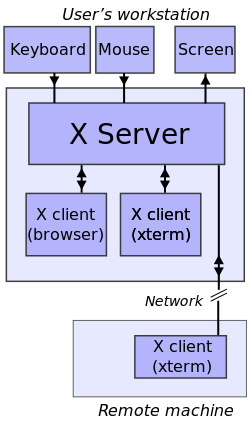
\includegraphics[width=0.6\linewidth]{xArchitecture}}
\caption{Архитектура протокола X}
\label{fig:xArchitecture}
\end{figure}

X использует модель клиент-сервер: сервер X взаимодействует с различными клиентскими программами. Сервер принимает запросы на графический вывод (окна) и отправляет обратно пользовательский ввод (с клавиатуры, мыши или сенсорного экрана). Сервер может работать как: 
\begin{itemize}
\item Приложение, отображающее окно другой системы отображения
\item Системная программа, управляющая видеовыходом ПК
\item Выделенный набор аппаратных средств
\end{itemize}

X рассматривает перспективу приложения, а не конечного пользователя: X предоставляет приложениям дисплей для отображения и пользовательский ввод-вывод приложениям, поэтому он является сервером; приложения используют эти службы, поэтому они являются клиентами. 

Протокол связи между сервером и клиентом работает прозрачно: клиент и сервер могут работать на одном компьютере или на разных устройствах, возможно, с разными архитектурами и операционными системами. Клиент и сервер могут даже безопасно обмениваться данными через Интернет путем туннелирования соединения по зашифрованному сетевому сеансу. Сам клиент X может эмулировать X-сервер, предоставляя услуги отображения другим клиентам. Это называется "X-вложенность". Клиенты с открытым исходным кодом, такие как Xnest и Xephyr, поддерживают такую ​​вложенность X.

Протокол X в первую очередь определяет примитивы протокола и графики --- он преднамеренно не содержит спецификаций для дизайна пользовательского интерфейса приложения. Вместо этого прикладные программы --- такие как оконные менеджеры, инструментальные средства GUI-виджета и среды рабочего стола или графические пользовательские интерфейсы приложений --- определяют и предоставляют такие детали. В результате нет типичного интерфейса X, и несколько различных сред настольных компьютеров стали популярными среди пользователей. Оконный менеджер контролирует размещение и внешний вид окон приложений.  Оконные менеджеры различаются по сложности и объемноси от самых простых (например, twm, основной оконный менеджер, поставляемый с X, или evilwm, чрезвычайно легкий оконный менеджер) в более комплексные среды рабочего стола, такие как Enlightenment. Основной идеей оконного менеджера в протоколе X является то, что ОМ не является непосредственной частью сервера, это клиентское приложение с некоторыми дополнительными возможностями. Для стандартизации протокола общения между ОМ и остальными клиентами, был разработан протокол ICCCM (Inter-Client Communication Conventions Manual)~\cite{icccm}, X Window System, обеспечивающий интероперабельность X-клиентов в пределах одного и того же X-сервера.

Когда оконный менеджер запущен, некоторые виды взаимодействия между X-сервером и его клиентами перенаправляются через оконный менеджер. В частности, всякий раз, когда делается попытка показать новое окно, этот запрос перенаправляется в ОМ, который определяет начальную позицию окна. Кроме того, большинство современных оконных менеджеров являются репарентирующими, что обычно приводит к размещению баннера в верхней части окна и оформлению декоративной рамки вокруг окна. Эти два элемента управляются оконным менеджером, а не программой. Поэтому, когда пользователь нажимает или перетаскивает эти элементы, именно оконный менеджер выполняет соответствующие действия (например, перемещение или изменение размера окна).

Менеджеры окон также отвечают за конки приложений. Когда пользователь запрашивает окно для его изменения, ОМ удаляет его (делает его невидимым) и предпринимает соответствующие действия, чтобы показать иконку на своем месте. 

Хотя главной задачей ОМ является управление окнами, многие оконные менеджеры имеют дополнительные функции, такие как обработка щелчков мыши в корневом окне, представление панелей и других визуальных элементов, обработка некоторых нажатий клавиш (например, Alt-F4 может закрыть окно ).

X-сервер состоит из набора расширений, каждое из которых реализует определённые функции: от прорисовки геометрических примитивов до ускорения обработки и вывода на экран трёхмерной графики с использованием возможностей видеоаппаратуры. Почти каждый из этих модулей можно отключить или настроить в конфигурационном файле.

\subsection{Протокол Wayland}
Wayland --- это протокол организации графического сервера в UNIX-подобных ОС и его библиотечная реализация на языке C~\cite{Wayland}. Так же протокол имеет свою референсную реализацию Weston~\cite{Weston}. Архитектура протокола Wayland приведена на рисунке~\ref{fig:waylandArchitechture}.

\begin{figure}[h!]
\center{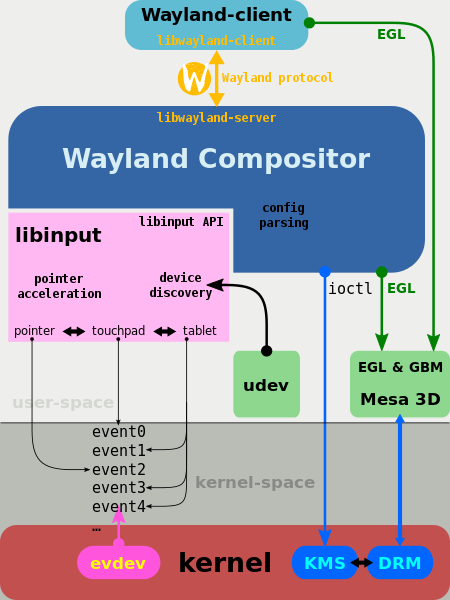
\includegraphics[width=0.7\linewidth]{waylandArchitechture}}
\caption{Архитектура протокола Wayland}
\label{fig:waylandArchitechture}
\end{figure}

Можно увидеть, что Wayland является клиент-серверным протоколом, в котором клиентами являются графические приложения, а сервером является композитор. Композитор --- это дисплейный сервер, который взаимодействует с пользовательскими устройствами ввода-вывода, с аппаратурой компьютера и управляет потоками данных клиентских приложений. В конечном счете, графические приложения запрашивают у сервера отображения своих графических буферов на экране, а композитор контролирует отображение этих буферов на экране. 

Реализация Wayland была разработана как двухслойный протокол (рис. \ref{fig:waylandClientServer}):
\begin{itemize}
\item Низкоуровневый протокол, который управляет межпроцессным взаимодействием между процессами клиента и композитора. Данный слой реализован с использованием средств ярда UNIX.
\item Поверх него построен высокоуровневый протокол, который обрабатывает информацию, которой должны обмениваться клиент и композитор для реализации базовый возможностей графической оболочки. 
\end{itemize}
\begin{figure}[h!]
\center{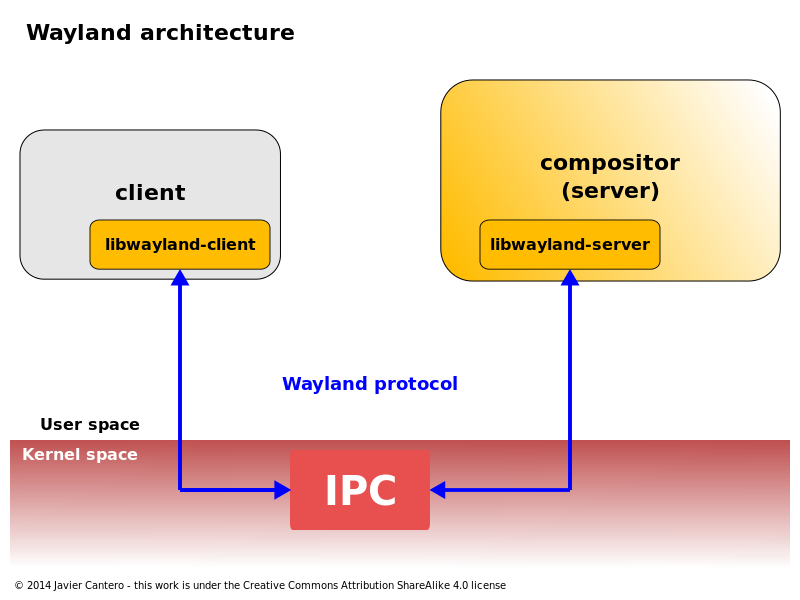
\includegraphics[width=0.7\linewidth]{waylandClientServer}}
\caption{Двухуровневая организация Wayland}
\label{fig:waylandClientServer}
\end{figure}

Реализация протокола Wayland разделена на две библиотеки: \texttt{libwayland-client} для клиентских приложений и \texttt{libwayland-server} для реализации композиторов.

Протокол Wayland описывается как "асинхронный объектно-ориентированный протокол". Объектно - ориентированность означает, что сервисы, предлагаемые композитором, представлены в виде набора объектов. Каждый объект реализует интерфейс, который имеет имя, ряд методов (называемых запросами), а также несколько связанных событий. Каждый запрос и событие имеет ноль или более аргументов, каждый из которых имеет имя и тип данных. Протокол является асинхронным в том смысле, что запросы не должны ждать синхронизированных ответов, избегая времени задержки на двустороннее сканирование. Таким образом достигается улучшенная производительность. 

Клиенты Wayland могут сделать запрос (вызов метода) для некоторого объекта, если интерфейс объекта поддерживает этот запрос. Клиент также должен предоставить необходимые данные для аргументов такого запроса. Именно так клиенты запрашивают сервисы у композитора. Композитор, в свою очередь, отправляет информацию клиенту, вызывая генерацию необходимых событий объекта. Эти события могут быть вызваны композитором как ответ на определенный запрос или асинхронно, в ответ на возникновение каких-либо внутренних событий (например, активность одного из устройства ввода). 

Для того, чтобы клиент мог сделать запрос к объекту, ему сначала нужно указать серверу идентификационный номер, который он будет использовать для идентификации этого объекта. В наборе данных есть два типа объектов: глобальные и локальные. Глобальные объекты указываются композитором клиентам, когда они созданы (а также когда они уничтожены), в то время как локальные объекты обычно создаются другими объектами, которые уже существуют как часть их функциональности. Интерфейсы, их запросы и события являются основными элементами, определяющими протокол Wayland. Каждая версия протокола включает в себя набор интерфейсов, а также их запросы и события, которые ожидаются в любом наборе Wayland. Опционально, Wayland композитор может определять и реализовывать свои собственные интерфейсы, которые поддерживают новые запросы и события, тем самым расширяя функциональность за пределами основного протокола.

Интерфейсы текущей версии протокола Wayland определены в файле протокола \texttt{protocol/wayland.xml} исходного кода Wayland. Это XML файл, в котором перечислены существующие интерфейсы текущей версии, а также их запросы, события и другие атрибуты. Этот набор интерфейсов является минимальным, необходимым для любого композитора Wayland. Некоторые из основных интерфейсов протокола Wayland:
\begin{itemize}
\item \texttt{wl\_display} --- основной глобальный объект, специальный объект для инкапсуляции самого протокола Wayland
\item \texttt{wl\_registry} --- глобальный объект реестра, в котором композитор регистрирует все глобальные объекты, которые он хочет предоставить клиентам
\item \texttt{wl\_compositor} --- объект, который представляет собой композитор, и отвечает за объединение различных буферов в один вывод
\item \texttt{wl\_surface} --- объект, представляющий прямоугольную область на экране, определяемую местоположением, размером и буфером пикселей
\item \texttt{wl\_buffer} --- объект, который при подключении к объекту \texttt{wl\_surface} предоставляет его отображаемое содержимое
\item \texttt{wl\_output} --- объект, представляющий отображаемую область экрана
\item \texttt{wl\_pointer, wl\_keyboard, wl\_touch} --- объекты, представляющие различные устройства ввода
\end{itemize} 

Типичный сеанс клиента Wayland начинается с открытия соединения с композитором с использованием объекта \texttt{wl\_display}. Это специальный локальный объект, который представляет соединение и не живет на сервере. Используя его интерфейс, клиент может запросить глобальный объект \texttt{wl\_registry} из композитора, где живут все глобальные имена объектов, и связывать те, что интересует клиента. Обычно клиент связывает по крайней мере объект \texttt{wl\_compositor}, откуда он будет запрашивать один или несколько объектов \texttt{wl\_surface} для отображения вывода приложения на дисплее.

Композитор Wayland может определять и экспортировать свои собственные дополнительные интерфейсы. Эта функция используется для расширения протокола за пределами базовых функций, предоставляемых основными интерфейсами, и стала стандартным способом реализации расширений протокола Wayland.

Для Wyaland так же существует расширение XWayland, которое позволяет запускать X-приложения в Wayland.

\subsection{Сравнение X и Wayland}
Существует несколько отличий между Wayland и X в отношении производительности, поддержки кода и безопасности: 
\begin{itemize}
\item Архитектура: композитор --- это отдельная дополнительная функция в X, а Wayland объединяет дисплейный сервер и композитор как единую функцию. Кроме того, он включает в себя некоторые из задач оконного менеджера, который в X является отдельным процессом на стороне клиента. 
\item Рендеринг: X-сервер по-умолчанию сам выполняет рендеринг окон. Существуют так же расширения позволяющие ему окно отрендеренное на стороне клиента. Напротив, Wayland по-умолчанию не предоставляет API для визуализации, а делегирует клиентам такие задачи (включая рендеринг шрифтов, виджетов и т. д.). Декорирование окон может выполняться на клиентской стороне (например, с помощью набора графических средств) или на стороне сервера (в функциональности композитора). 
\item Безопасность: Wayland изолирует входные и выходные данные каждого окна, обеспечивая конфиденциальность, целостность и доступность в обоих случаях; X не имеет этих важных функций безопасности. Кроме того, с подавляющим большинством кода, работающего на клиенте, меньше кода нужно запускать с правами root, что повышает безопасность. 
\item Межпроцессное взаимодействие: X-сервер предоставляет базовый метод обмена между X-клиентами, позднее расширенный протоколом ICCM. Это взаимодействие X клиент --- X клиент используется менеджерами окон, для реализации X-сессий, функций drag-and-drop, а многих других функций. Основной протокол Wayland не поддерживает связь между wayland-клиентами вообще, и соответствующая функциональность (если необходимо) должна быть реализована в окружении рабочего стола (например, KDE или GNOME) или третьей стороной (например, используя IPC базовая операционной системы).
\item Сетевое взаимодействие: X --- это архитектура, изначально разработанная для работы по сети. Wayland не предлагает сетевой прозрачности сам по себе, однако, композитор может реализовать любой протокол удаленного рабочего стола для достижения удаленного отображения. Кроме того, существуют исследования потоковой передачи и сжатия изображений Wayland, которые обеспечивали бы доступ к буферу буфера удаленного доступа, подобный VNC.
\end{itemize}

На основе всех этих фактов можно сказать, что Wayland является более современной графической средой, в которой учтены и исправлены многие ошибки X. Благодаря этому, Wayland так же выигрывает у X в производительности. Wayland так же поддерживает X-приложения (через XWayland). Таким образом, можно сделать вывод, что наиболее оптимальным выбором для реализации своего мобильного оконного менеджера будет выбор Wayland.
